\documentclass[10pt, twoside, a4paper, openright]{report}

%packages-----------------------------------------------------------------------

\usepackage[utf8]{inputenc}
\usepackage[english]{babel}
\usepackage[T1]{fontenc}
\usepackage{lmodern}
\usepackage{array}
%\usepackage{times}
%\usepackage{charter}
\usepackage{graphicx}
\usepackage{color}
\usepackage{amsmath}
\usepackage{amssymb}
\usepackage{amsthm}
\usepackage{verbatim}
\usepackage{pdfpages}
\usepackage[unicode]{hyperref}
\hypersetup{
	colorlinks=true,
	urlcolor=blue,
	linkcolor=blue,
	citecolor=blue
}
\newcommand{\link}[3][blue]{\href{#2}{\color{#1}{#3}}}%
\usepackage[small, bf]{caption}
\usepackage{enumerate}
\usepackage{epstopdf}
\usepackage{epsfig}
\usepackage{setspace}
\usepackage{esdiff}
\usepackage{enumitem}
\usepackage[inner=4.0cm, outer=3.0cm]{geometry}
\usepackage{emptypage}
\usepackage{caption}
%\usepackage{subcaption}
\usepackage{listings}
\usepackage{multicol}
\usepackage{multirow}
\usepackage{lipsum}
\usepackage{mathabx}
\usepackage{floatrow}
\usepackage{courier}
\usepackage{cite}
\def\citepunct{; \penalty\citepunctpenalty}
\usepackage[position=top]{subfig}
%\usepackage[autostyle]{csquotes}

\newcommand{\q}[1]{``#1''} % quotation marks

%cite----------



%fancystyles--------------------------------------------------------------------

\usepackage{fancyhdr}

\fancypagestyle{myfancy}{

\fancyhead[LE]{\nouppercase{\leftmark}}
\fancyhead[LO]{}
\fancyhead[CO]{}
\fancyhead[CE]{}
\fancyhead[RE]{}
\fancyhead[RO]{\nouppercase{\rightmark}}

\fancyfoot[LE]{\thepage}
\fancyfoot[LO]{}
\fancyfoot[CO]{}
\fancyfoot[CE]{}
\fancyfoot[RE]{}
\fancyfoot[RO]{\thepage}

\renewcommand{\headrulewidth}{0.4pt}
\renewcommand{\footrulewidth}{0.0pt}
}

\fancypagestyle{plain}{

\fancyhead[LE]{}
\fancyhead[LO]{}
\fancyhead[CO]{}
\fancyhead[CE]{}
\fancyhead[RE]{}
\fancyhead[RO]{}

\fancyfoot[LE]{\thepage}
\fancyfoot[LO]{}
\fancyfoot[CO]{}
\fancyfoot[CE]{}
\fancyfoot[RE]{}
\fancyfoot[RO]{\thepage}

\renewcommand{\headrulewidth}{0.0pt}
\renewcommand{\footrulewidth}{0.0pt}
}

%tikz---------------------------------------------------------------------------

\usepackage{tikz}
\usetikzlibrary{shapes, arrows}

%url----------------------------------------------------------------------------

\usepackage{url}
\DeclareUrlCommand\url{\def\UrlLeft{<}\def\UrlRight{>} \urlstyle{tt}}

%color--------------------------------------------------------------------------

\definecolor{darkred}{rgb}{0.6,0,0}
\definecolor{darkgreen}{rgb}{0,0.6,0}
\definecolor{darkblue}{rgb}{0,0,0.6}
\definecolor{darkgrey}{rgb}{0.3,0.3,0.3}
\definecolor{grey}{rgb}{0.6,0.6,0.6}
\definecolor{lightgrey}{rgb}{0.95,0.95,0.95}
\definecolor{lightred}{rgb}{0.99,0.85,0.85}
\definecolor{violet}{rgb}{0.65,0.45,0.75}

%listings-----------------------------------------------------------------------

\definecolor{mygreen}{rgb}{0,0.6,0}
\definecolor{mygray}{rgb}{0.5,0.5,0.5}
\definecolor{light}{rgb}{0.96, 0.96, 0.96}
\definecolor{mymauve}{rgb}{0.58,0,0.82}

\lstdefinestyle{CXX} {
	language=C++,
	backgroundcolor=\color{light},
	basicstyle=\scriptsize\ttfamily,
	breakatwhitespace=false,
	breaklines=true,
	captionpos=t,
	%commentstyle=\color{mygreen},
	deletekeywords={},
	escapeinside={\%*}{*)},
	extendedchars=true,
	frame=single,
	keepspaces=true,
	keywordstyle=\color{blue},
	otherkeywords={},
	numbers=left,
	numbersep=5pt,
	numberstyle=\tiny\color{mygray},
	rulecolor=\color{black},
	showspaces=false,
	showstringspaces=false, 
	showtabs=false,
	stepnumber=1,
	stringstyle=\color{mymauve},
	tabsize=3,
	title=\lstname   
}

\lstdefinestyle{FORTRAN} {
	language=[90]Fortran,
	backgroundcolor=\color{light},
	basicstyle=\scriptsize\ttfamily,
	keywordstyle=\color{blue},
	%commentstyle=\color{mygreen},
	breakatwhitespace=false,
	breaklines=true,
	captionpos=t,
	deletekeywords={},
	escapeinside={\%*}{*)},
	extendedchars=true,
	frame=single,
	keepspaces=true,
	otherkeywords={},
	numbers=left,
	numbersep=5pt,
	numberstyle=\tiny\color{mygray},
	rulecolor=\color{black},
	showspaces=false,
	showstringspaces=false, 
	showtabs=false,
	stepnumber=1,
	stringstyle=\color{mymauve},
	tabsize=3,
	title=\lstname 
}

%settings-----------------------------------------------------------------------

\setlength{\parindent}{15pt}
\setlength{\parskip}{0pt}
\renewcommand{\baselinestretch}{1.0}
\pagenumbering{arabic}
\frenchspacing

\DeclareFontFamily{U}{mathx}{\hyphenchar\font45}
\DeclareFontShape{U}{mathx}{m}{n}{<-> mathx10}{}
\DeclareSymbolFont{mathx}{U}{mathx}{m}{n}
\DeclareMathAccent{\widebar}{0}{mathx}{"73}

%commands----------------------------------------------------------------------

\newcommand{\ctu}{Czech Technical University in Prague}
\newcommand{\fnspe}{Faculty of Nuclear Sciences and Physical Engineering}
\newcommand{\dpe}{Department of Physical Electronics}
\newcommand{\branch}{Computational Physics}
\newcommand{\projecttitle}{Laser-driven sources of~electrons and~x-rays in~underdense plasma: theory and~simulation}
\newcommand{\projecttitlecz}{Laserem řízené zdroje elektronů a~rentgenového záření v~podkritickém plazmatu: teorie a~simulace}
\newcommand{\valenta}{Ing. Petr Valenta}
\newcommand{\klimo}{doc. Ing. Ondřej Klimo, Ph.D.}
\newcommand{\bulanov}{prof. Sergei Vladimirovich Bulanov}
%\newcommand{\year}{2022}
\newcommand{\keywords}{}
\newcommand{\keywordscz}{}

%macros-------------------------------------------------------------------------

\newcommand{\nucl}[3]{
\ensuremath{
\phantom{
\ensuremath{^{#1}_{#2}}}
\llap{\ensuremath{^{\rule{0pt}{0pt}#1}}}
\llap{\ensuremath{_{\rule{0pt}{7pt}#2}}}
\mbox{#3}}}

\newcommand{\norm}[1]{\lVert#1\rVert}
\newcommand{\abs}[1]{\lvert#1\rvert}

\renewcommand{\vec}[1]{\mathbf{#1}}

\newcommand{\rot}[1]{\nabla \times #1}
\newcommand{\grad}[1]{\nabla #1}
\renewcommand{\div}[1]{\nabla \cdot #1}
\newcommand{\laplace}[1]{\Delta #1}
\newcommand{\dalembert}[1]{\Box #1}

\newcommand{\e}[0]{\mathrm{e}}
\renewcommand{\i}[0]{\mathrm{i}}
\renewcommand{\d}[0]{\mathrm{d}}

%changecountering---------------------------------------------------------------

\usepackage{chngcntr}
%\counterwithout{equation}{chapter}
\counterwithout{figure}{chapter}
\counterwithout{table}{chapter}

%document-----------------------------------------------------------------------

\begin{document}

\pagestyle{empty}

%1------------------------------------------------------------------------------

\mbox{}
\newpage

\begin{titlepage}

\begin{center}
\epsfysize=35mm \epsffile{img/logo/ctu.pdf} \\[15mm]
\end{center}

\begin{center}
\begin{spacing}{2.0}
{\rule{125mm}{2pt}} \\[4mm]
{\huge \bf \projecttitle} \\
{\rule{125mm}{2pt}} \\[5mm]
\end{spacing}
{\LARGE by Petr Valenta} \\
\end{center}

\vfill

\begin{center}
\parbox{0.75\textwidth}{\noindent \centering \large Dissertation submitted to the \\ \fnspe, \\ \ctu, \\ in partial fulfillment of the requirements for the degree of Doctor of Philosophy.}
\end{center}

\vfill

\begin{center}
{\large Prague, 2022}
\end{center}

\end{titlepage}

%2------------------------------------------------------------------------------

\newpage
\rule{0pt}{0pt}
\vfill
\begin{description}
	\item[supervisor:]\ \\
	\klimo \\
	\fnspe, \\ 
	\ctu, \\
	Břehová 7, 115 19 Prague, \\
	Czech Republic
\end{description}

\begin{description}
	\item[supervisor specialist:]\ \\
	\bulanov \\
	Institute of Physics, \\
	Czech Academy of Sciences, \\
	Na Slovance 1999/2, 182 21 Prague, \\
	%Za Radnicí 835, 252 41 Dolní Břežany, \\
	Czech Republic
\end{description}
\vglue 1cm

\noindent Copyright {\copyright} {2022} {Petr Valenta}

%3------------------------------------------------------------------------------

%\newpage
%\includepdf[pages=1]{dat/guidelines.pdf}

%4------------------------------------------------------------------------------

%\newpage
%\includepdf[pages=2]{dat/guidelines.pdf}

%5------------------------------------------------------------------------------

%\newpage
%\null
%\vfill
%{\bf \noindent Prohlášení/Declaration} \\[5mm]
%Prohlašuji, že jsem předloženou práci vypracoval samostatně a že jsem uvedl veškerou
%použitou literaturu.\\[2mm]
%I hereby declare that I carried out this work independently, and only with the cited sources, literature and other professional sources.\\
%\vspace{5mm}V Praze dne/In Prague on .............................\hfill
%\begin{tabular}{c}
%........................................\\
%\valenta
%\end{tabular}

%6------------------------------------------------------------------------------

%\newpage
%\thispagestyle{empty}
%\mbox{}

%7------------------------------------------------------------------------------

%\newpage
%\begin{flushleft}
%	\renewcommand{\arraystretch}{1.3}
%	\begin{tabular}{r p{12cm}}
%		Název práce:
%		~ & \bf \projecttitlecz \\
%		Autor:
%		~ & \valenta \\
%		Druh práce:
%		~ & Diplomová práce \\
%		Studijní program:
%		~ & (N3913) Aplikace přírodních věd \\
%		Obor:
%		~ & (3901T065) Informatická fyzika \\
%		Vedoucí práce:
%		~ & \klimo \newline Katedra fyzikální elektroniky, Fakulta jaderná a fyzikálně inženýrská, České vysoké učení technické v Praze \\
%		Konzultant:
%		~ & \bulanov \newline Projekt ELI-Beamlines, Fyzikální ústav Akademie věd České republiky, v. v. i. \\
%	\end{tabular}
%\end{flushleft}

%\begin{center}
%\textbf{Abstrakt}\\
%\end{center}

%Úzká fokusace s využitím plazmové optiky může vést ke zvýšení intenzity a zlepšení časového i prostorového kontrastu laserových svazků. Vzhledem k tomu, že pro popis těchto impulsů neplatí paraxiální aproximace, je zapotřebí použít vhodnější model. V rámci této práce byly do částicového kódu implementovány a důkladně otestovány nové okrajové podmínky pro výpočet časového vývoje laserového impulsu na hranici simulační obasti v souladu s Maxwellovými rovnicemi. Upravený kód byl použit pro simulace laserových svazků zaostřených do velmi malého ohniska. Výsledky simulací byly analyzovány z hlediska vlivu velikosti ohniska na průběh interakce laserových svazků s pevnými terči. Ukazuje se, že trajektorie horkých elektronů a absorpční procesy během interakce jsou silně ovlivněny příčnou složkou ponderomotorické síly, která je velmi vysoká v případě ohniska menšího než je vlnová délka laseru. V tomoto případě ostře narůstá účinnost absorpce laserové energie v plazmatu, distribuční funkce energie elektronů jsou kvalitativně rozdílné a teplota horkých elektronů se výrazně zvyšuje. \\

%\noindent Klíčová slova: \keywordscz


%8------------------------------------------------------------------------------

\newpage
\pagestyle{myfancy}

\chapter*{Abstract \markboth{Abstract}{Abstract}}
\addcontentsline{toc}{chapter}{Abstract}

We explore novel regimes of laser-plasma interaction accessible by new generation laser systems. The scientific focus is mainly devoted to enhancement of laser-generated sources of accelerated electrons and coherent short-wavelength radiation based on plasma waves driven by intense laser pulses. First we describe mechanisms for obtaining electron beams based on laser wakefield acceleration technique. We analyze the properties of the wakefield in regimes dominated by the effects of dispersion and carrier envelope phase. Discussed range of parameters is relevant for electron acceleration at high repetition rate. Second we investigate the concept of relativistic mirrors in laser plasmas. We describe the recoil effects on reflection from relativistic mirrors which is crucial for maximizing the energy of reflected radiation. We find the threshold for incident pulse energy above which the relativistic mirrors undergo significant back reaction. We also analyze the generation of coherent hard electromagnetic radiation by the reflection from the electron density singularities.\\

{\noindent \bf Keywords:} laser-plasma interaction, laser wakefield acceleration, relativistic mirrors, short-wavelength radiation \keywords

\newpage
\thispagestyle{empty}
\mbox{}

%9------------------------------------------------------------------------------

\tableofcontents
\addtocontents{toc}{\protect\thispagestyle{empty}}
\thispagestyle{empty}

%-------------------------------------------------------------------------------

\chapter{Introduction}
%\addcontentsline{toc}{chapter}{Introduction}
%\input{dat/introduction.tex}

\section{Aims and motivation / objectives of the thesis / problem statement}
%\input{dat/1-0.tex}

\section{Originality and contributions / role of author}
%\input{dat/1-0.tex}

\section{Related work / previous results / state-of-the-art}
%\input{dat/1-0.tex}

\section{Outline of the thesis / structure}
%\input{dat/1-0.tex}

%-------------------------------------------------------------------------------

\chapter{Physics of laser-underdense plasma interaction}
%\input{dat/1-0.tex}

\section{Equations of EM field}
%\input{dat/1-0.tex}

\section{EM waves in vacuum}
%\input{dat/1-0.tex}

\section{Gaussian beam optics}
%\input{dat/1-0.tex}

\section{Interaction with single electrons, ponderomotive force}
The relativistic motion of an electron in the presence of transverse electromagnetic wave 

\section{Langmuir waves, wave breaking, catastrophe theory}
%\input{dat/1-0.tex}

\section{Self-focusing, self-guiding, self-phase modulation, self-amplitude modulation}
%\input{dat/1-0.tex}

%-------------------------------------------------------------------------------

\chapter{Laser-wakefield acceleration of electrons}
%\input{dat/1-0.tex}

\section{Electron interaction with Langmuir wave}
\input{src/electron_interaction_with_langmuir_wave.tex}

\section{Electron injection mechanisms}
%\input{dat/1-0.tex}

\subsection{Injection by breaking plasma wave}
%\input{dat/1-0.tex}

\subsubsection{Homogeneous plasma}
%\input{dat/1-0.tex}

\subsubsection{Inhomogeneous plasma}
%\input{dat/1-0.tex}

\subsection{Optical injection}
%\input{dat/1-0.tex}

\subsection{Ionization injection}
%\input{dat/1-0.tex}

\section{Regimes of LWFA}
%\input{dat/1-0.tex}

\subsection{Self-modulated regime}

\subsection{Blow-out regime}

\section{Limitations of LWFA}
%\input{dat/1-0.tex}

\subsection{Electron dephasing length}

\subsection{Pump depletion length}

\subsection{Beam loading}

\section{Applications of accelerated electrons}
%\input{dat/1-0.tex}

%-------------------------------------------------------------------------------

\chapter{Relativistic mirrors}
%\input{dat/1-0.tex}

\section{Lorentz transform, Doppler effect}
%\input{dat/1-0.tex}

\subsection{Uniformly moving mirror}
%\input{dat/1-0.tex}

\subsection{Accelerated mirror}
%\input{dat/1-0.tex}

\subsection{Oscillating mirror}
%\input{dat/1-0.tex}

\section{Physical realization of relativistic mirrors in underdense plasma}
%\input{dat/1-0.tex}

\subsection{Langmuir wave}
%\input{dat/1-0.tex}

\subsection{Bow wave}
%\input{dat/1-0.tex}

%-------------------------------------------------------------------------------

\chapter{Numerical methods}
%\input{dat/1-0.tex}

\section{Particle-in-cell algorithm}
%\input{dat/1-0.tex}

%-------------------------------------------------------------------------------

\chapter{Author's original results}
%\input{dat/1-0.tex}

In this chapter, the reader can find an overview of the main results achieved within the author's postgraduate studies. In total, we select four papers published in peer-reviewed journals which are fully (or from the most part) based on the author's original work. Below, we provide a brief summary of each selected paper as well as a detailed description of the author's role and contributions. Full texts of all the selected publications are enclosed in Appendix~\ref{chap:selected_publications}.

\section{On the electromagnetic-electron rings}
%\input{dat/1-0.tex}

First, we present the results of research devoted to the coupled electromagnetic and electron rings originating from the interaction of high-power short-pulse laser and underdense plasma, which has been published in Ref.~\citenum{bibid} (the reader can find the full text of the paper in Appendix~\ref{sec:paper_1}). This research has been initiated after the experimental observation of stable and tunable ring-shaped beams of high-energy electrons; the experiment has been carried out by the ELI Beamlines Electron Acceleration Group at the Institute of Plasma Physics and Laser Microfusion in Warsaw, Poland (the reader can find further details in Ref.~\citenum{Grittani2018}). Our preliminary goal was to find out and describe the underlying physical mechanisms which lead to the formation of ring-shaped electron beams in laser plasmas. Although several mechanisms that may result in the electron rings of similar parameters were already identified and presented in literature at that time (see, e.g., Refs.~\citenum{Kaganovich2008, Zhang2012, Pollock2015, Zhao2016, Yang2017, Behm2019, Salehi2021}), none of them seemed to correspond to the particular experimental parameters used in Ref.~\citenum{Grittani2018}.

In general, this work investigates (analytically and using numerical simulations) the propagation of high-power short-pulse laser in a low-density plasma, which is a topic relevant to a number of scientific challenges, such as laser-driven acceleration of charged particles \cite{Tajima1979, Esarey2009, Gonsalves2019}, development of sources of hard electromagnetic radiation \cite{Pirozhkov2012, Bulanov2013}, and nuclear fusion within the framework of the fast ignition concept \cite{Tabak1994}. For many of these applications, it is essential that the laser pulse propagates over extended distances and transmits its energy into the plasma in controlled way without incurring excessive losses. In this context, much of the attention has been focused on the evolution of the radial profile of the laser beam in a fully ionized plasma; it turned out that the process of self-focusing for high-power laser pulses may lead to the formation of the multifilament and, in particular, ring-shaped transverse structures \cite{Mori1988, Cohen1991, Borisov1992, Krushelnick1997, Cattani2001, Kim2002, Naseri2016, Kovalev2019}. We show that these electromagnetic rings can become a source of high-energy ring-shaped electron beams. 

In addition to the applications mentioned above, the understanding of the physical processes that lead to the generation of the electromagnetic and electron ring structures is important due to the following reasons: (i) the electromagnetic rings may carry off a significant fraction of energy from the driver, and thus limit the overall efficiency of applications based on the laser-plasma interaction; (ii) the electron beams accelerated in the wake of the electromagnetic rings may cause a damage to surrounding equipment (e.g., capillaries used for the laser pulse guiding) and become a source of unwanted electromagnetic radiation; and (iii) the knowledge of the origin of the electromagnetic and electron rings could serve as a diagnostics for determining the regimes of laser-plasma interaction.

The first part of the paper presents an analytical model based on geometric optics approximation which qualitatively illustrates the origin and the initial stage of the electromagnetic ring formation. We define the plasma density distribution within the Langmuir wave as well as the Hamiltonian for the photon interaction with the Langmuir wave; the trajectories of photons are then obtained by solving the Hamilton equations. The second part of the paper presents a three-dimensional particle-in-cell simulation, the results of which demonstrate the formation of the electromagnetic as well as electron ring. We discuss the mechanism of formation of the electromagnetic ring and the processes of electron injection into the accelerating phase of the secondary wakefield generated by the electromagnetic ring. Finally, the third part of the paper contains the results of a systematic multi-parametric simulation study for various plasma densities, laser intensities, and laser spot sizes revealing the relationships among the properties of the electromagnetic rings and the parameters of laser and plasma.

The main results of the paper can be summarized as follows. We identify and describe a novel physical mechanism which leads to the formation of ring-shaped electromagnetic-electron structures, where the electromagnetic rings arise from the laser pulse defocusing induced by the excitation of Langmuir waves in underdense plasma, and the ring-shaped electron beams are formed and accelerated subsequently by the secondary toroidal wakefields generated by the electromagnetic rings. We further reveal that the electromagnetic rings are relatively robust nonlinear objects, whose properties can be controlled by tuning the parameters of laser and plasma. Within the studied parameter range, we find that up to $ \approx 70 \ \% $ of the total initial driver pulse energy can be carried off by the electromagnetic rings having the opening angles $ \approx 50 - 105 \ \mathrm{mrad} $. 

Besides Ref.~\citenum{bibid}, a portion of this work has been also published in Ref.~\citenum{bibid} and presented by the author at \q{SPIE Optics+Optoelectronics 2021}, \q{OPTO2021 Symposium on Photon and Beam Science}, and \q{ELI Summer school 2021}, whereas the latter presentation has been awarded by the \q{Best poster prize}. The author contributed to all the aspects of the research, including the initial formulation of the scientific topic, development of the analytical model, setup and execution of the numerical simulations on computer clusters, and analysis and interpretation of the simulation data. Furthermore, based on the results obtained the author prepared figures and wrote the bulk of the manuscript text, submitted the manuscript to the journal whereas serving as a corresponding author, and was communicating with editors and referees until the final publication in the journal.

\section{On the laser-wakefield polarity reversal}
%\input{dat/1-0.tex}

Second, we present the results of research devoted to the laser-wakefield acceleration of electrons in the regime of ultrashort pulses and near-critical density plasmas, which has been published in Ref.~\citenum{Valenta2020b} (the reader can find the full text of the paper in Appendix~\ref{sec:paper_2}). This research is closely related to the laser-wakefield acceleration of electrons driven by high-repetition-rate ($ \gtrsim \mathrm{kHz} $) laser systems (such as the L1 laser system at ELI Beamlines). 

The research on laser-wakefield acceleration of electrons has been predominantly oriented on the Joule-class laser systems, which have already demonstrated their capability to produce electron beams at the multi-$ \mathrm{GeV} $ energy scale with a relative energy spread of a few percent \cite{Kim2013, Gonsalves2019}, a few $ \mathrm{fs} $ duration \cite{Tilborg2006, Ohkubo2007, Debus2010, Lundh2011}, and hundreds of $ \mathrm{pC} $ of charge \cite{Li2017, Couperus2017} (although not simultaneously). Recently, however, there has been a growing interest in the laser-wakefield acceleration of electrons driven by high-repetition-rate ($ \gtrsim \mathrm{kHz} $) laser systems since they can significantly improve certain characteristics (e.g., stability, signal-to-noise ratio, and average electron current \cite{Faure2018}) required by a number of practical applications (e.g., ultrafast electron diffraction \cite{Sciaini2011, Miller2014}, $ \mathrm{fs} $ x-ray generation \cite{TaPhuoc2012, Corde2013}, and pulsed radiolysis \cite{Muroya2008}). On the other hand, present-day high-repetition-rate lasers deliver (due to the constraints in technology) pulses with energy of only a few $ \mathrm{mJ} $. This (together with the requirements of the blow-out regime of the laser-wakefield acceleration) implies that, in order to produce high-quality relativistic electron sources, one has to use tightly-focused near-single-cycle pulses and thin near-critical density gas targets \cite{Faure2018, Salehi2019}. Such considerations constitute a great challenge not only from a technical point of view, but also in the sense of the understanding of underlying physical processes (e.g., related to the $ \lambda^{3} $ regime \cite{Mourou2002}).

In the first part of the paper we extend the standard model of the wakefield generation by considering the carrier-envelope phase shift of the driving laser pulse. The model shows that wakefield contains long-wavelength modulation of its amplitude. In the second part of the paper we analytically investigate the acceleration of single relativistic electron by the modulated wakefield. We show that the electron energy gain depends on the initial phase of the driver and find the case for which the net energy acquired by the electron over given distance is maximal. Finally, the third part of the paper contains the setup and the results of the three-dimensional particle-in-cell simulation on the self-consistent evolution of the ultrashort laser pulse and near-critical density plasma. The simulation results are in qualitative agreement with the analytical model.

The main results of the paper can be summarized as follows. We reveal for the first time (to the best of our knowledge) that the wakefield, being excited by an ultrashort laser pulse in plasma, periodically reverses its polarity. As shown by the analytical model and numerical simulation, the wakefield polarity reversal is caused by dispersion and the corresponding difference between the propagation speed of the carrier and the envelope of the driving laser pulse. Further, we show that the novel phenomenon of the wakefield polarity reversal occurs on spatial scales shorter than the dephasing length and, therefore, significantly affects the energy spectra of accelerated electron beams. In the nonlinear regime, however, there may exist a case for which the polarity reversal length is equal to the dephasing length. In such a case, the dephasing limit is overcome and the electrons are accelerated until the energy of the driver pulse depletes. The discovery of this phenomenon is crucial for better control of the parameters of electron beams accelerated via the laser-wakefield mechanism (e.g., by adjusting the initial phase of the driver or by controlling the phase of the electron injection), particularly in experiments carried out with present-day high-repetition-rate laser systems.

Besides Ref.~\citenum{Valenta2020b}, a portion of this work has been also published in Refs.~[Lazzarini + book, SPIE, EPS] and presented by the author at \q{ELI Users' conference 2020}, \q{SPIE Optics+Optoelectronics 2019}, and \q{EPS Conference on Plasma Physics 2018}, whereas the latter presentation has been awarded by the \q{Best poster prize}. The author contributed to all the aspects of the research, including the initial formulation of the scientific topic, development of the analytical model, setup and execution of the numerical simulations on computer clusters, and analysis and interpretation of the simulation data. Furthermore, based on the results obtained the author prepared figures and wrote the bulk of the manuscript text, submitted the manuscript to the journal whereas serving as a corresponding author, and was communicating with editors and referees until the final publication in the journal.

\section{On the recoil effects of relativistic mirrors}
%\input{dat/1-0.tex}

Third, we present the results of research devoted to the sources of coherent short-wavelength radiation based on the concept of relativistic flying mirrors in plasma, which has been published in Ref.~\citenum{valenta2020} (the reader can find the full text of the paper in Appendix~\ref{sec:paper_3}). This work investigates (analytically and using numerical simulations) the recoil effects associated with the interaction of relativistic mirrors and strong counter-propagating electromagnetic waves as well as the properties of the reflected radiation.

Relativistic mirrors in plasmas are actively studied as a unique tool for fundamental research (e.g., light intensification toward the Schwinger limit, investigation of photon–photon and Delbruck scattering, analog black hole to investigate Hawking radiation, and the information loss paradox) and for many practical applications in diverse fields; depending on whether the configuration is co-propagating or counter-propagating in the laboratory frame of reference, relativistic mirrors might be used either for the acceleration of ions (e.g., for hadron therapy) or for producing coherent high-brightness radiation with wavelengths ranging from x-ray to gamma-ray (e.g., for molecular imaging and attosecond spectroscopy).

The first part of the paper 

Particularly, we consider a relativistic mirror in a form of strongly nonlinear Langmuir wave.

and the cohow a strong electromagnetic wave incident on the relativistic mirror affects the motion of the mirror and the corresponding recoil effects.

amplification and frequency up-shift factors.

This research reveals that if the fluence of the electromagnetic wave incident on the relativistic mirror exceeds a certain threshold, the relativistic mirror undergoes a back reaction significantly affecting its amplification and frequency up-shift factors.



\section{On the relativistic flying forcibly oscillating mirror}
%\input{dat/1-0.tex}

The last publication introduces a novel scheme of the relativistic flying mirrors

%-------------------------------------------------------------------------------

\chapter{Conclusions}
%\addcontentsline{toc}{chapter}{Conclusion and forthcoming work}
%\input{dat/conclusion.tex}

\section{Summary}

\section{Perspectives}

%\newpage
%\pagestyle{plain}
%\null
%\vfill
%{\bf \noindent Acknowledgments} \\

%I wish express my gratitude to both, my supervisor \klimo and consultant \bulanov for constant support and guidance, as well as for providing invaluable advice and direction.\\

%Access to computing and storage facilities owned by parties and projects contributing to the National Grid Infrastructure MetaCentrum, provided under the programme "Projects of Large Infrastructure for Research, Development, and Innovations" (LM2010005), is greatly appreciated.\\

%Access to the CERIT-SC computing and storage facilities provided under the programme Center CERIT Scientific Cloud, part of the Operational Program Research and Development for Innovations (reg. no. CZ.1.05/3.2.00/08.0144) is greatly  appreciated.\\

%This work was supported by the project ELI: Extreme Light Infrastructure (reg. no. CZ.02.1.01/0.0/0.0/15\_008/0000162) from European Regional Development.\\

%The development of the EPOCH code was funded in part by the UK EPSRC grants EP/G054950/1, EP/G056803/1, EP/G055165/1 and EP/M022463/1.\\
%\begin{flushright}
%\valenta
%\end{flushright}

\newpage

\chapter*{Acknowledgements \markboth{Acknowledgements}{Acknowledgements}}
\addcontentsline{toc}{chapter}{Acknowledgements}

%-------------------------------------------------------------------------------

\newpage
\addcontentsline{toc}{chapter}{Bibliography}
\bibliographystyle{bib/my-apalike}
\bibliography{bib/references}

%-------------------------------------------------------------------------------

\part*{Appendices \markboth{Appendices}{Appendices}}
\addcontentsline{toc}{chapter}{Appendices}

\appendix

\chapter{List of author's publications \label{chap:authors_publications}}

Below, the reader can find the list of publications in peer-reviewed journals, conference proceedings, and book chapters authored or co-authored by the author during the author's postgraduate studies. The publications are listed in chronological order.

\section{Publications in peer-reviewed journals \label{sec:peer_reviewed_journals}}

\begin{itemize}
	
	\item Mu, J., Esirkepov, T. Z., \underline{Valenta, P.}, Jeong, T. M., Gu, Y., Koga, J. K., Pirozhkov, A. S., Kando, M., Korn, G., and Bulanov, S. V. (2019). \link{http://dx.doi.org/10.3103/S1541308X19040010}{High-order harmonics from laser irradiated electron density singularity formed at the bow wave in the laser plasma}. \textit{Physics of Wave Phenomena}, \textbf{27}(4):247-256.
	
	\item \underline{Valenta, P.}, Esirkepov, T. Z., Koga, J. K., Pirozhkov, A. S., Kando, M., Kawachi, T., Liu, Y. K., Fang, P., Chen, P., Mu, J., Korn, G., Klimo, O., and Bulanov, S. V. (2020). \link{http://dx.doi.org/10.1063/1.5142084}{Recoil effects on reflection from relativistic mirrors in laser plasmas}., \textit{Physics of Plasmas}, \textbf{27}(3):032109.
	
	\item Esirkepov, T. Z., Mu, J., Gu, Y., Jeong, T. M., \underline{Valenta, P.}, Klimo, O., Koga, J. K., Kando, M., Neely, D., Korn, G., Bulanov, S. V., and Pirozhkov, A. S. (2020). \link{http://dx.doi.org/10.1063/5.0004525}{Optical probing of relativistic plasma singularities}. \textit{Physics of Plasmas}, \textbf{27}(3):052103.
	
	\item Mu, J., Esirkepov, T. Z., \underline{Valenta, P.}, Gu, Y., Jeong, T. M., Pirozhkov, A. S., Koga, J. K., Kando, M., Korn, G., and Bulanov, S. V. (2020). \link{http://dx.doi.org/10.1103/PhysRevE.102.053202}{Relativistic flying forcibly oscillating reflective diffraction grating}. \textit{Physical Review E}, \textbf{102}(5):053202.
	
	\item \underline{Valenta, P.}, Esirkepov, T. Z., Koga, J. K., Nečas, A., Grittani, G. M., Lazzarini, C. M., Klimo, O., Korn, G., and Bulanov, S. V. (2020). \link{http://dx.doi.org/10.1103/PhysRevE.102.053216}{Polarity reversal of wakefields driven by ultrashort pulse laser}. \textit{Physical Review E}, \textbf{102}(5):053216.
	
	\item Hadjisolomou, P., Jeong, T. M., \underline{Valenta, P.}, Korn, G., and Bulanov, S. V. (2021). \link{http://dx.doi.org/10.1103/PhysRevE.104.015203}{Gamma-ray flash generation in irradiating a thin foil target by a single-cycle tightly focused extreme power laser pulse}. \textit{Physical Review E}, \textbf{104}(1):015203.
	
\end{itemize}

\section{Publications in conference proceedings \label{sec:conference_proceedings}}

\begin{itemize}
	
	\item Klimo, O., \underline{Valenta, P.}, and Weber, S. (2017). \link{http://ocs.ciemat.es/EPS2017PAP/pdf/P5.225.pdf}{Laser absorption and ion acceleration under tight-focusing conditions}. \textit{44th EPS Conference on Plasma Physics}, P5.225.
	
	\item \underline{Valenta, P.}, Klimo, O., Bulanov, S. V., and Korn, G. (2018). \link{http://ocs.ciemat.es/EPS2018PAP/pdf/P2.2031.pdf}{On high-quality electron beam generated by breaking wake wave in near-critical density plasmas}. \textit{45th EPS Conference on Plasma Physics}, P2.2031. 
	
	\item \underline{Valenta, P.}, Klimo, O., Grittani, G. M., Esirkepov, T. Z., Korn, G., and Bulanov, S. V. (2019). \link{http://dx.doi.org/10.1117/12.2521040}{Wakefield excited by ultrashort laser pulses in near-critical density plasmas}. \textit{Proc. SPIE 11037, Laser Acceleration of Electrons, Protons, and Ions V}, 110370T.
	
	\item Mu, J., Gu, Y., Jeong, T. M., \underline{Valenta, P.}, Klimo, O., Esirkepov, T. Z., Pirozhkov, A. S., Koga, J. K., Kando, M., Korn, G., and Bulanov, S. V. (2019). \link{http://dx.doi.org/10.1117/12.2524653}{High order harmonics generation via laser reflection at electron density peaks}. \textit{Proc. SPIE 11039, Research Using Extreme Light: Entering New Frontiers with Petawatt-Class Lasers IV}, 110390H.
	
	\item Lazzarini, C. M., Goncalves, L. V., Grittani, G. M., Lorenz, S., Nevrkla, M., \underline{Valenta, P.}, Levato, T., Bulanov, S. V., and Korn, G. (2020). \link{http://dx.doi.org/10.1142/S0217751X19430103}{Electron acceleration at ELI Beamlines: towards high-energy and high-repetition-rate accelerators}. \textit{International Journal of Modern Physics A}, \textbf{34}(34):1943010.
	
	\item \underline{Valenta, P.}, Esirkepov, T. Z., Koga, J. K., Pirozhkov, A. S., Kando, M., Kawachi, T., Liu, Y. K., Fang, P., Chen, P., Mu, J., Korn, G., Klimo, O., and Bulanov, S. V. (2020). \link{http://dx.doi.org/10.1364/EUVXRAY.2020.EM1A.5}{Relativistic flying mirrors as a compact source of coherent short-wavelength radiation}. \textit{OSA High-brightness Sources and Light-driven Interactions Congress 2020}, EM1A.5.
	
	\item \underline{Valenta, P.}, Grittani, G. M., Lazzarini, C. M., Klimo, O., and Bulanov, S. V. (2021). \link{http://dx.doi.org/10.1117/12.2589222}{Ring-shaped electron beams from laser-wakefield accelerator}. \textit{Proc. SPIE 11779, Laser Acceleration of Electrons, Protons, and Ions VI}, 1177909.
	
	\item Jeong, T. M., Bulanov, S. V., \underline{Valenta, P.}, Korn, G., Esirkepov, T. Z., Koga, J. K., and Pirozhkov, A. S (2021) \link{http://dx.doi.org/10.1117/12.2592047}{Ultra-strong attosecond laser focus produced by a relativistic-flying parabolic mirror}. \textit{Proc. SPIE 11886, International Conference on X-Ray Lasers 2020}, 118860H.
	
\end{itemize}

\section{Book chapters \label{sec:book_chapters}}

\begin{itemize}
	
	\item Matys, M., Pšikal, J., Danielová, M., \underline{Valenta, P.}, and Bulanov, S. V. (2019). \link{https://www.it4i.cz/cs/file/abd1875ff7d0e6f59799c4f470545516/173/Supercomputing-in-Science-and-Engineering_preview.pdf}{Laser-driven ion acceleration using cryogenic hydrogen targets}. \textit{Supercomputing in Science and Engineering 2017-18}, pp. 149-151.
	
	\item Lazzarini, C. M., Goncalves, L. V., Grittani, G. M., Lorenz, S., Nevrkla, M., \underline{Valenta, P.}, Levato, T., Bulanov, S. V., and Korn, G. (2020) \link{http://dx.doi.org/10.1142/9789811217135_0010}{Electron acceleration at ELI Beamlines: towards high-energy and high-repetition-rate accelerators}. \textit{Beam Acceleration in Crystals and Nanostructures}, pp. 153-170.
	
	\item Matys, M., \underline{Valenta, P.}, Kecová, M., Nishihara, K., Pšikal, J., Esirkepov, T. Z., Koga, J. K., Nečas, A., Grittani, G. M., Lazzarini, C. M., Klimo, O., Korn, G., and Bulanov, S. V. (2021). \link{}{Laser-driven acceleration of charged particles}. \textit{Supercomputing in Science and Engineering 2019-20}, pp. xxx-xxx.
	
\end{itemize}

\chapter{Selected publications \label{chap:selected_publications}}
%\input{dat/appendix_a.tex}

\section{On the electromagnetic-electron rings originating from the interaction of high-power short-pulse laser and underdense plasma \label{sec:paper_1}}

In this section, the reader can find the full text of Valenta, P., Esirkepov, T. Zh., Koga, J. K., Pirozhkov, A. S., Kando, M., Kawachi, T., Liu, Y. K., Fang, P., Chen, P., Mu, J., Korn, G., Klimo, O., and Bulanov, S. V. (2020). \link{http://dx.doi.org/10.1063/1.5142084}{Recoil effects on reflection from relativistic mirrors in laser plasmas}., \textit{Physics of Plasmas}, \textbf{27}(3):032109.

\newpage
\mbox{}
\thispagestyle{empty}

\newpage
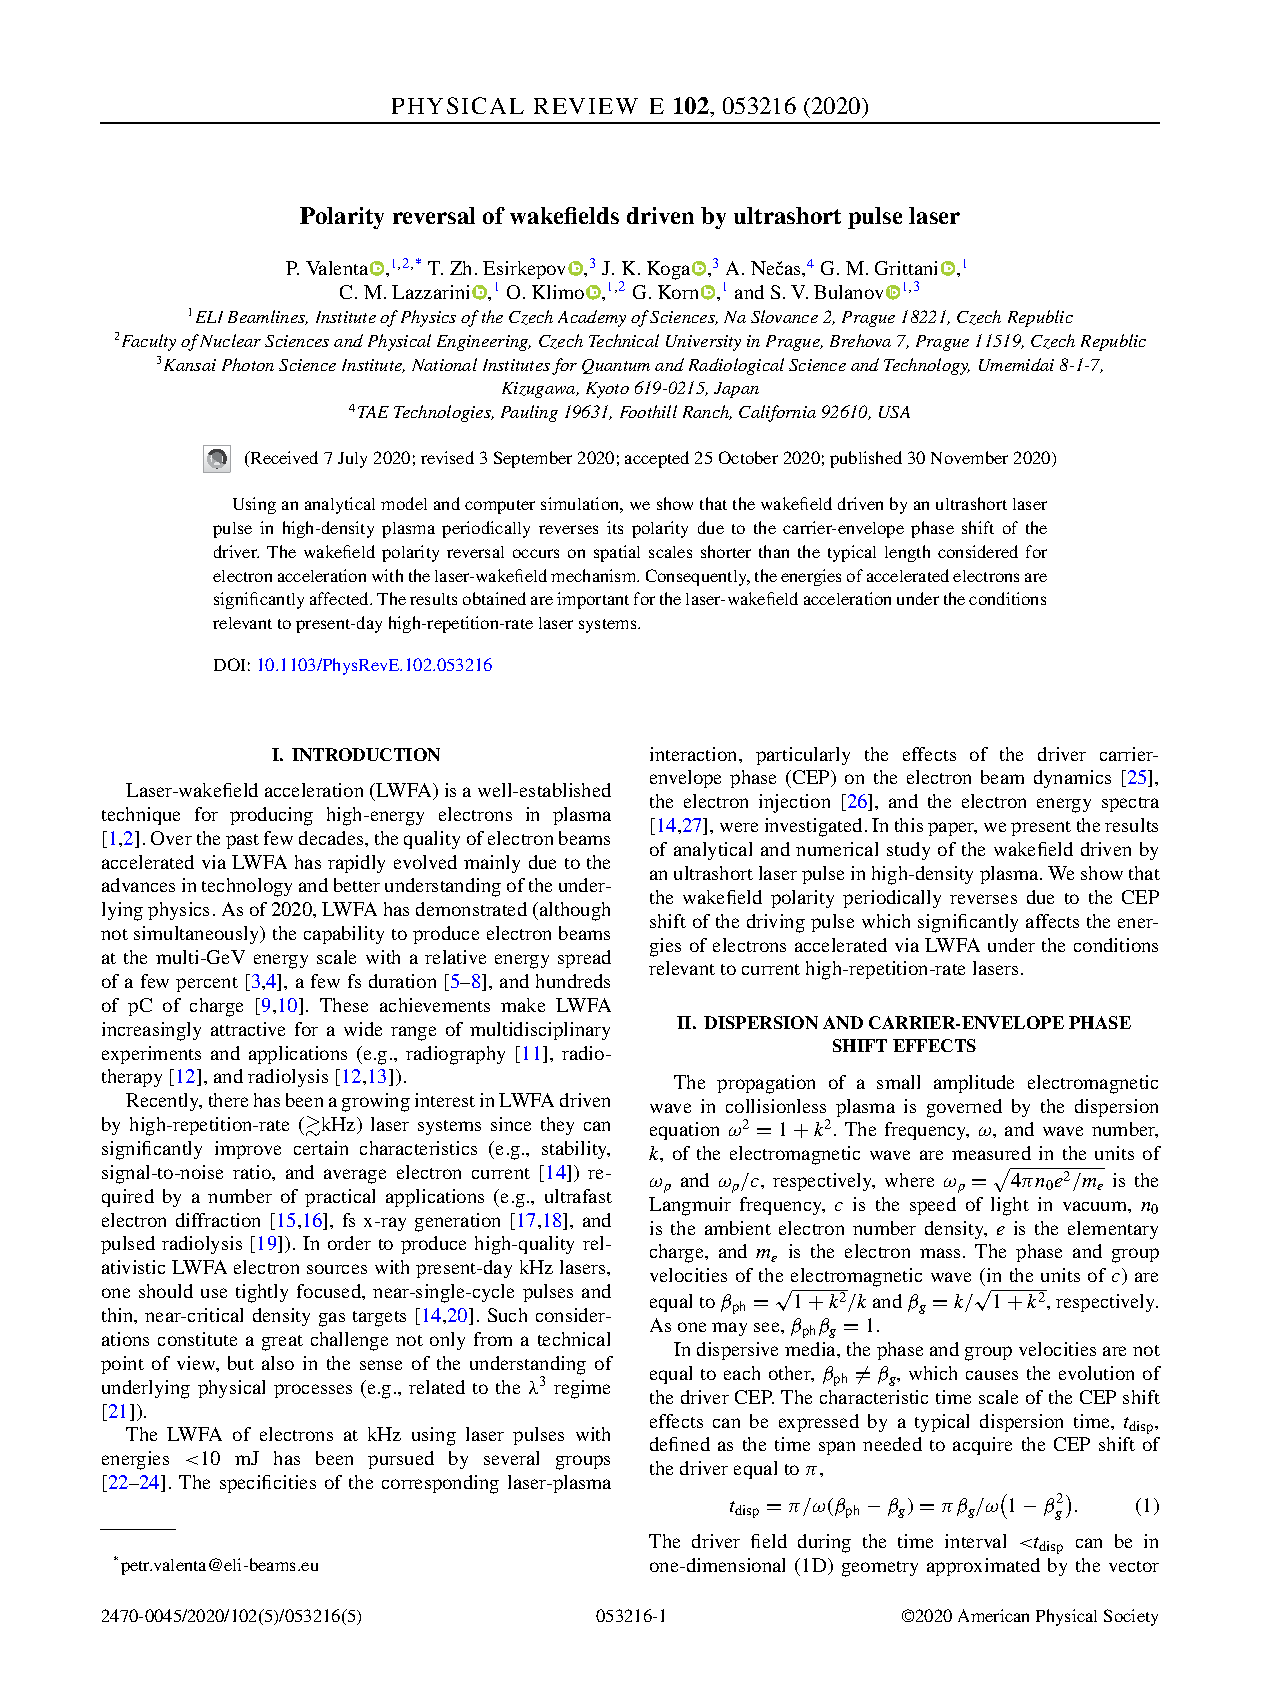
\includepdf[pages=-]{misc/paper2.pdf}

\newpage
\mbox{}
\thispagestyle{empty}

\newpage
\section{Polarity reversal of wakefields driven by ultrashort pulse laser \label{sec:paper_2}}

In this section, the reader can find the full text of Valenta, P., Esirkepov, T. Zh., Koga, J. K., Nečas, A., Grittani, G. M., Lazzarini, C. M., Klimo, O., Korn, G., and Bulanov, S. V. (2020). \link{http://dx.doi.org/10.1103/PhysRevE.102.053216}{Polarity reversal of wakefields driven by ultrashort pulse laser}. \textit{Physical Review E}, \textbf{102}(5):053216.

\newpage
\mbox{}
\thispagestyle{empty}

\newpage
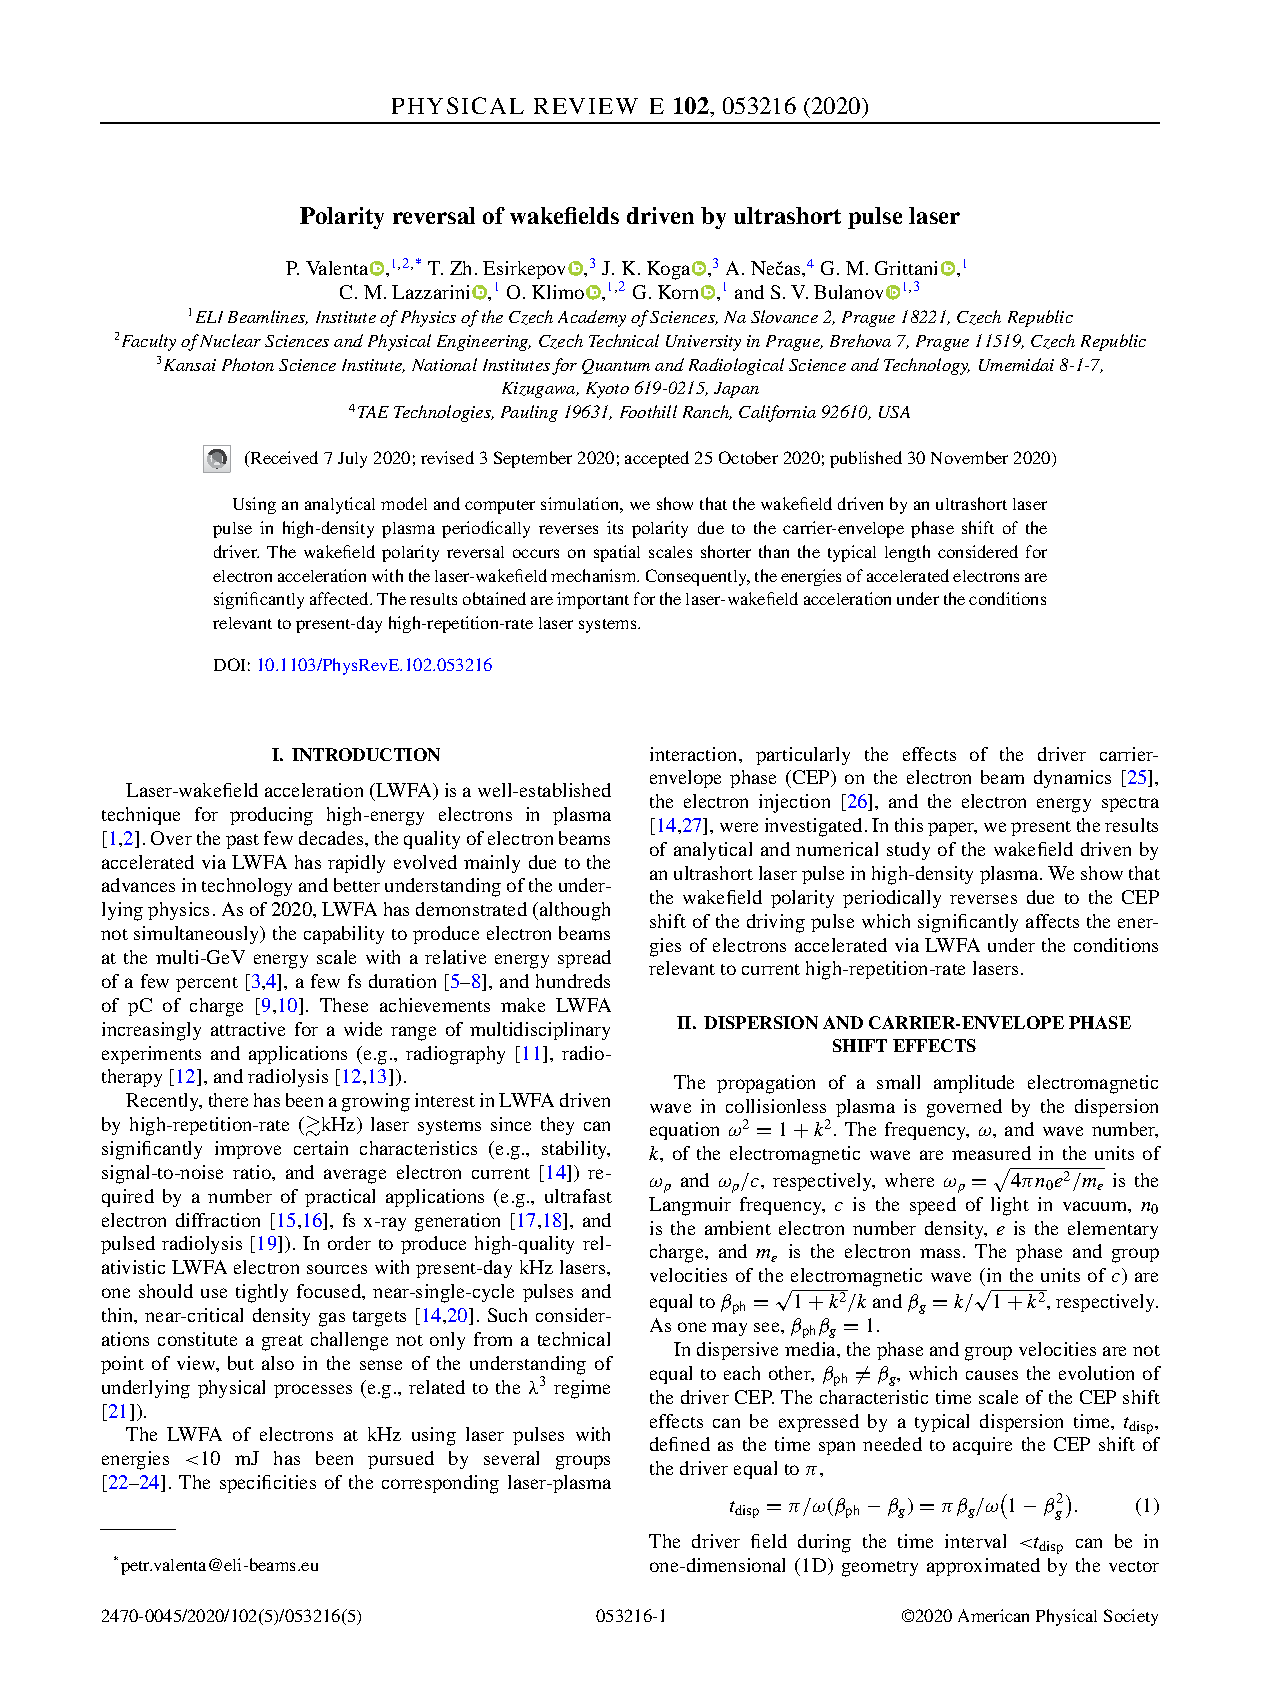
\includepdf[pages=-]{misc/paper2.pdf}

\section{Recoil effects on reflection from relativistic mirrors in laser plasmas \label{sec:paper_3}}

In this section, the reader can find the full text of Valenta, P., Esirkepov, T. Zh., Koga, J. K., Pirozhkov, A. S., Kando, M., Kawachi, T., Liu, Y.-K., Fang, P., Chen, P., Mu, J., Korn, G., Klimo, O., and Bulanov, S. V. (2020). \link{http://dx.doi.org/10.1063/1.5142084}{Recoil effects on reflection from relativistic mirrors in laser plasmas}., \textit{Physics of Plasmas}, \textbf{27}(3):032109.

\newpage
\includepdf[pages=2-]{misc/paper3.pdf}

\mbox{}
\thispagestyle{empty}
\newpage


\section{Relativistic flying forcibly oscillating reflective diffraction grating \label{sec:paper_4}}

In this section, the reader can find the full text of Mu, J., Esirkepov, T. Zh., Valenta, P., Gu, Y., Jeong, T. M., Pirozhkov, A. S., Koga, J. K., Kando, M., Korn, G., and Bulanov, S. V. (2020). \link{http://dx.doi.org/10.1103/PhysRevE.102.053202}{Relativistic flying forcibly oscillating reflective diffraction grating}. \textit{Physical Review E}, \textbf{102}(5):053202.

\newpage
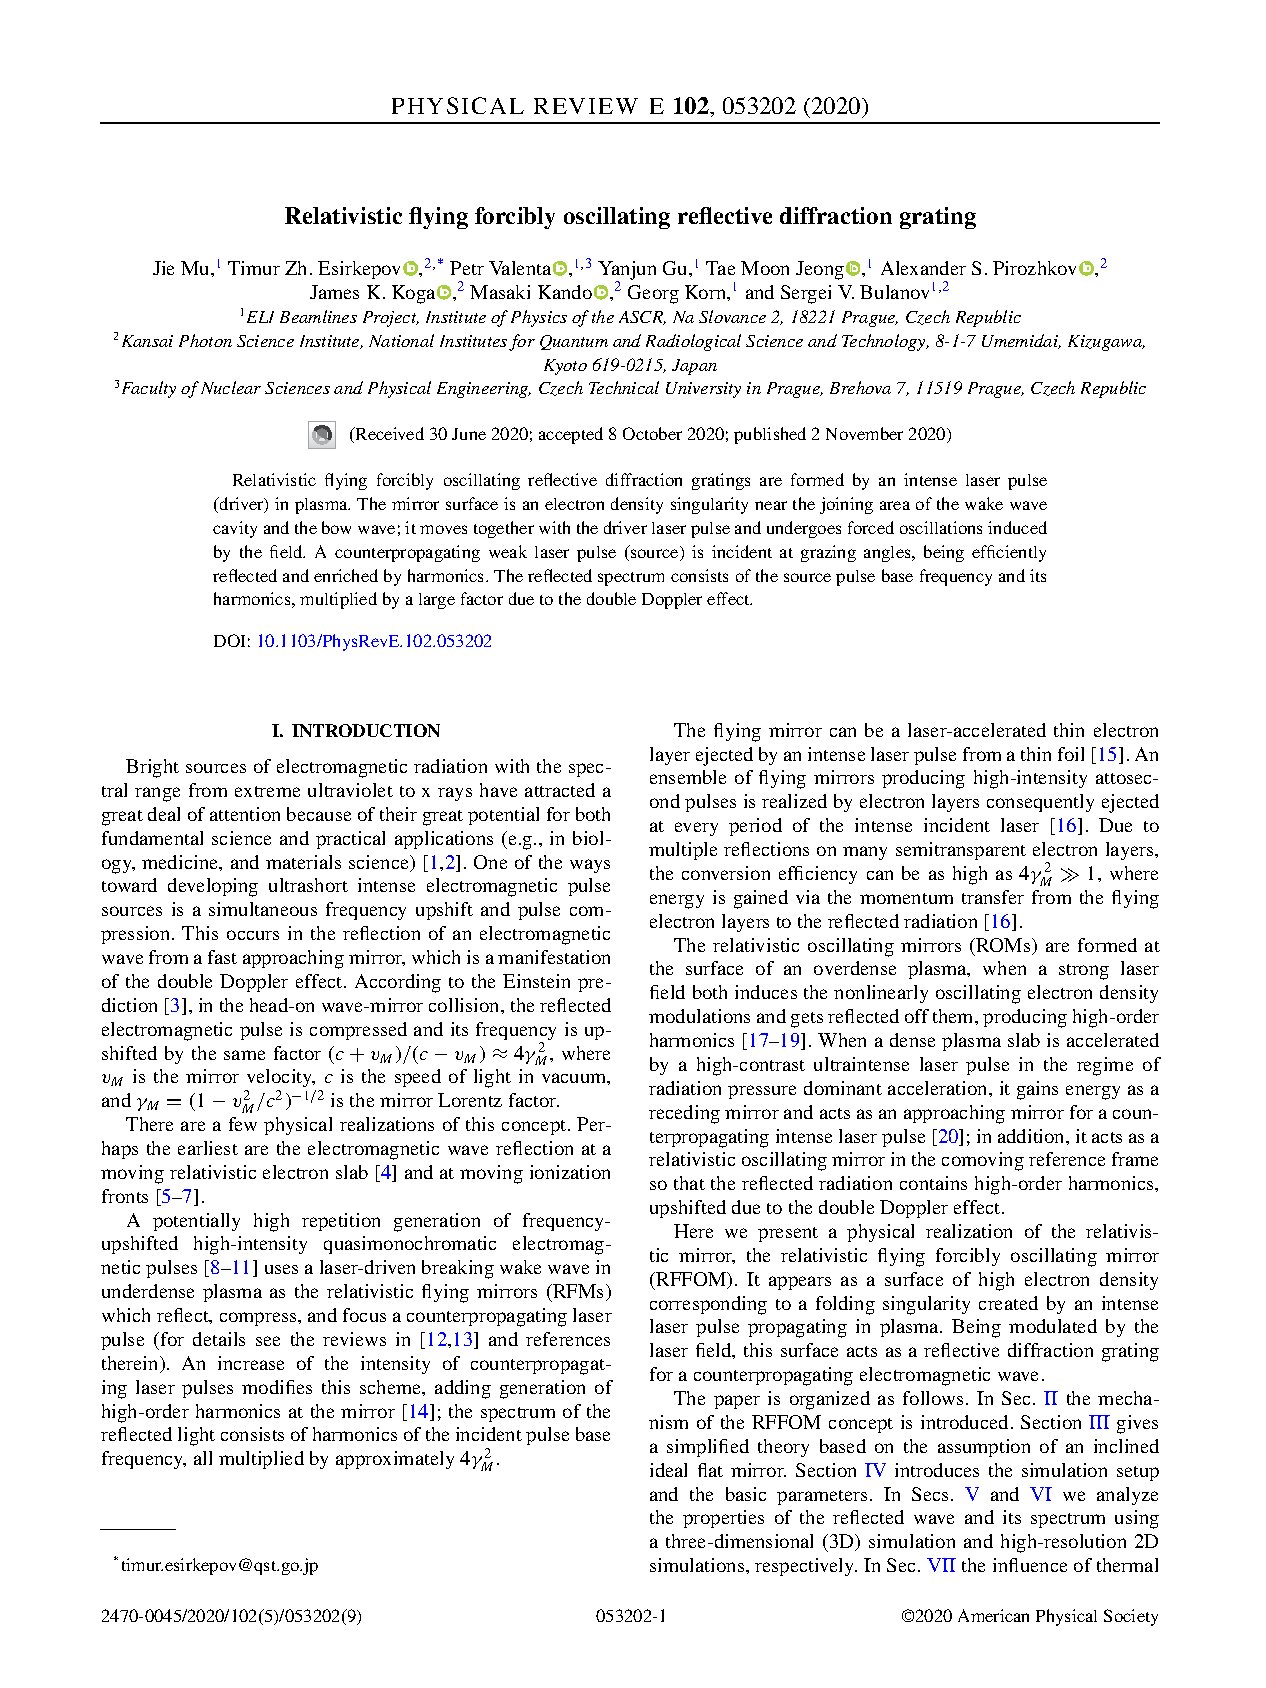
\includepdf[pages=-]{misc/paper4.pdf}

%\chapter{Code listings}
%\input{dat/appendix_b.tex}

%\chapter{CD content}
%\input{dat/appendix_c.tex}

\end{document}